\subsection{CoAtNet}

\paragraph{Entrenamiento desde cero (scratch + normalizado):}
CoAtNet, la arquitectura híbrida que integra capas convolucionales MBConv con módulos de atención Transformer, fue entrenada desde cero con el pipeline de normalización rigurosa durante 30 épocas. Las métricas de desempeño obtenidas se presentan en la Tabla~\ref{tab:coatnet_scratch_metrics}.

\begin{table}[H]
\centering
\caption{Métricas de CoAtNet entrenado desde cero con pipeline normalizado.}
\label{tab:coatnet_scratch_metrics}
\begin{tabular}{lc}
\hline
Métrica & Valor \\
\hline
Accuracy  & 98.35\% \\
Balanced Accuracy & 98.27\% \\
Precisión & 99.34\% \\
Recall (Sensibilidad) & 98.44\% \\
Especificidad & 98.10\% \\
F1-Score & 98.89\% \\
MCC & 0.9572 \\
AUC-ROC & 0.9952 \\
\hline
\end{tabular}
\end{table}

CoAtNet manifestó el rendimiento superior del estudio con 98.35\% de accuracy, excediendo a ViT-B/16 por 2.61 puntos porcentuales con 69\% menos parámetros (26.7M vs. 85.8M). La sinergia de convoluciones iniciales —que proporcionan sesgo inductivo de localidad— con atención global en etapas avanzadas generó el equilibrio óptimo entre capacidad representativa y eficiencia operacional. Las curvas de aprendizaje documentan una convergencia excepcionalmente rápida: en la época~3 el modelo ya superaba 96.62\% de exactitud en validación. El entrenamiento fue el más equilibrado de todas las arquitecturas evaluadas, con una diferencia train/val de solo 0.0000 en la época óptima (época~14, val\_loss de 0.0389), evidenciando ausencia total de sobreajuste paramétrico.

\begin{figure}[H]
\centering
    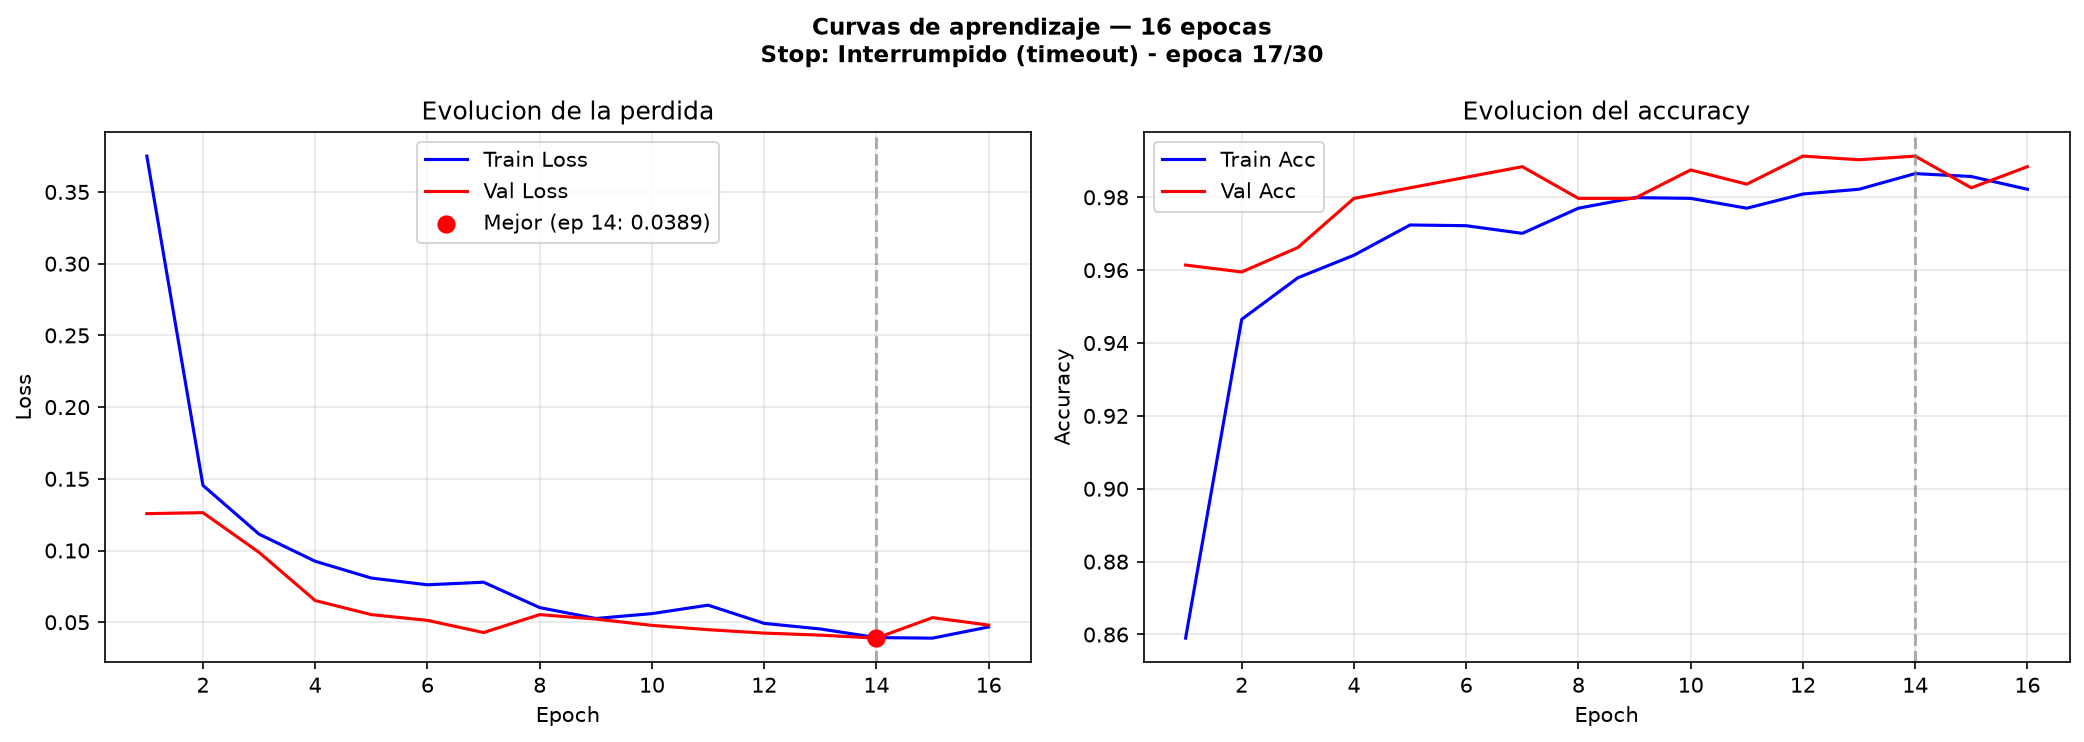
\includegraphics[width=0.95\columnwidth]{../BrainTumor/results/coatnet/normalized_scratch/learning_curves.png}
    \caption{Curvas de aprendizaje de CoAtNet desde cero con pipeline normalizado.}
    \label{fig:coatnet_scratch_lc}
\end{figure}
